% Skateboarding involves a human controlling a four wheeled vehicle that is steered by tilting the standing surface. The riding mechanics of skateboarding have been well reported [1][2]. The sport also includes aerial maneuvers such as jumping of stairs, flying off ramps and flipping and rotating the skateboard. The most basic aerial trick is called the ollie. The athlete jumps up while pushing down on the back end of the skateboard’s tail, causing a rotation about the back axle. The upward acceleration due to the rotation together with the tail-ground impact cause the skateboard to go airborne. Midair the athlete pulls the skateboard up through frictional contact and levels it out to land the trick. The most absolute performance measure of the trick is height [3]. To reach maximum height the dynamics such as impact, dynamic response, and torque production are dependent on shape, inertia and mass, which gives reason to assume an optimal shape exists. This leads to the research question: How do geometric parameters influence the maximum jumping height during the ollie. A 9-piece two-dimensional model is made with a theoretical inertia values. The inertia values are tested and scaled appropriately to verify the model. With a multi-phase direct collocation scheme the model is optimized for maximum height subject to the dynamics of the skater and human to find the optimal trajectory and parameters. The ollie height is improved by changing either one of these parameters relative to a standardized skateboard; longer wheelbase,  smaller tail angle, shorter flat part, and lower truck height.
% The results could be beneficial for Olympic performers to score higher points and push the sport to a new level. The method does not only apply to skateboarding, but any maneuver involving a human used artefact which has performance related dimensions. Such as, golf, honk ball, or cycling could be optimized similarly; model the artefact, simplify the input, set a performance metric, and optimize for optimal control and dimensions. 
\section{Introduction}\label{s_intro}
\noindent In 1978 Alan `Ollie' Gelfand invented the `no-hand aerial' in a bowl. Later Rodney Mullen was known for inventing the ollie from flat ground. The ollie, is a skateboard trick that intends to bring the skater with skateboard up. Because the skateboard is not tethered to the skater in any way, a precise sequence of movements is needed to keep the skater and skateboard together \cite{frederick_biomechanics_2006}. The maneuver can be described in six distinct phases which are shown in figure \ref{fig:ollie}. 

Throughout the history of skateboarding, multiple different skateboards have been developed for different pursuits. The first shape innovation was the the kicktail \cite{stevenson_skateboard_1971}, invented by Larry Stevenson in 1969. This particular shape enables the user to generate torque around the back wheels, to lift up the nose. This new shape was essential in performing an ollie to create upward acceleration of the board seen in the `pop' phase in fig. \ref{fig:ollie} C. 

By 1977, skateboarding branched into four distinct pursuits: downhill, slalom, freestyle, and bowl riding. For maximum performance in downhill riding the longboard was invented. A longboard is generally longer than 0.9 [m] for maximum stability \cite{prentiss_get_2011}. But this extended length does not help with the execution of an ollie, longboards are generally hard to ollie. In slalom, skateboards required speed and maneuverability, favoring shorter boards. In bowl riding, wider 0.25 [m] boards with high concavity were preferred for maximum foothold whilst riding vertical. Meanwhile, freestyle boards, designed for doing tricks on flat ground involved a kick-tail to quickly turn and twist. From these 4 distinct board shapes, new shapes evolved through a process of preference, resulting in functional and non-functional shapes \cite{prentiss_get_2011}. For example, non-functional developments were fish or coffins shaped decks with neon graphics and countless copyright infringements. Functional improvements resulted in the the `Popsicle Stick' skateboard. It evolved with the purpose of freestyle, with the ollie being the most basic trick. The `new' symmetrical shape also added the ability to use the nose for tricks. The popsicle stick skateboard is still the most widely used skateboard. All Olympic performers use a variation on this shape. 

The evolution resulted in skateboards being non-standard. Every brand uses their own measures for these dimensions \cite{berger_handmade_2021}. Typical dimensions of a professional skateboard are shown in the table \ref{tab:dimensions}. The dimensions of the skateboard are usually presented to the buyer with non specific descriptions such as mellow, steep, and wide. Deck dimensions are measured differently per brand\footnote{\url{http://skateboardingismylifetimesport.blogspot.com/2013/05/deck-length-measuring-by-company.html}}. This makes it difficult for skaters to find the deck of their preference.
\begin{figure}[t]
    \centering
        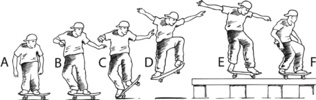
\includegraphics[width = 0.45\textwidth]{figure/f_ollie.png}
        \caption*{\centering \footnotesize Source: \cite{frederick_biomechanics_2006}}
        \caption[Ollie phases]{\footnotesize{(A)`Preparation': athlete lowers their centre of mass(COM) prepares muscles for upward acceleration. \\
        (B) `Pre-pop': skateboard rotates about it's wheels due to force of back foot. \\
        (C) `Pop': tail of the skateboard hits the ground. Skater takes advantage of the collision between the skateboard and ground to bring the skateboard up. \\
        (D) `Upward motion': the skater and skateboard are both airborne. \\
        (E) `Downward motion': the legs are extended to ensure a firm landing. \\
        (F) `Landing': the skater absorbs the impact. }}
        \label{fig:ollie}
\end{figure}

\begin{table}[b]
\begin{center} \label{table:dimensions}
\begin{tabular}{||c c||} 
 \hline
 Variable & Dimension range \\ [0.5ex] 
 \hline\hline
 Kick tail angle & 10-25 [deg]\\ 
 \hline
 Wheelbase & 0.30-0.50 [m]\\
 \hline
 Wheel diameter  & 48-60 [mm] \\
 \hline
 Truck height & 48-56 [mm] \\ 
 \hline
 Tail/nose length & 0.10-0.20[m] \\
 \hline
 Overall length & 0.74-0.85[m] \\
 \hline 
 Deck width& 0.19-0.22 [m] \\ [1ex] 
 \hline
\end{tabular}
\end{center}
    \caption[Typical dimension of a skateboard]{\centering Typical dimensions of a skateboard}
    \caption*{\centering \footnotesize Source: \cite{berger_handmade_2021}}
    \label{tab:dimensions}
\end{table}

Skaters know and feel when a specific skateboard performs to their liking. Though, they don’t know what dimensions support their performance. The skateboard might have evolved to an optimum throughout the years, but from an academical and mechanical point of view, skateboard design has not been proven optimal for specific tricks.

Some researches have tackled this problem by analyzing the skateboard in a planar riding model \cite{hubbard_lateral_1979,hubbard_human_1980,kremnev_nonlinear_2010,ispolov_skateboard_1996,rosatello_skateboard_2015,varszegi_stability_2017,varszegi_stabilizing_2016,varszegi_downhill_2016,varszegi_balancing_2014,kuleshov_mathematical_2007,kuleshov_various_2010}. Which has given insight in the dimensions and stability of rolling and turning. Researchers found that the stability of the skater with skateboard is dependent on the location, and input of the athlete, wheelbase, torsional spring stiffness of roll and forward speed \cite{varszegi_stability_2017,kremnev_nonlinear_2010,hubbard_lateral_1979}. These dimensional analyses don't apply to ollies. Others researched the ollie by investigating the contact forces \cite{anderson_ollie_2020,shield_contact-implicit_2022} and biomechanics \cite{frederick_biomechanics_2006,vorlicek_analysis_2015,wood_3d_2020,nakashima_simulation_2021,nevitt_ground_2006,candotti_lower_2012,dias_using_2016,anderson_ollie_2020,bridgman_human_1992,ou_postural_2021}. Two papers investigated the optimization of the ollie without changing the geometry \cite{anderson_ollie_2020,shield_contact-implicit_2022}. But research does not provide how the skateboards' dimensions influence the ollie. The skateboard community would benefit from knowing how the dimensions of the skateboard influence the performance of the ollie. 
Now that skateboarding joined the Olympics, knowing how to improve performance is more important then ever. The most concrete (i.e. criteria with physical measurement) Olympic judging criteria that applies to the ollie is height \cite{world_skate_skateboarding_2021}. I have parameterized the geometry and inertia characteristics of a skateboard modeled as a single rigid body with parameters: tail length, tail angle, deck length, truck height, and wheel radius. This is an appropriate parameterization for a skateboard designer because the width of the skateboard is usually chosen by preference. Also, the ollie is a movement that involves rotation in one plane, visible in fig. \ref{f_olliesteps}, which means only the inertia characteristics for this rotation are necessary. 
\newpage
\noindent This leads to the following research question:

\begin{quote}
\textit{
    What are the optimal geometric and inertial parameters of a skateboard for an Olympic athlete to reach maximal ollie height?}
\end{quote}

This paper aims to provide information to skaters on how the dimensions of the skateboard influence the ollie.\\ 
